\section{Measurement Principle and Mode}

Ultrasonic ranging can be implemented using several methods,
including pulse-echo time-of-flight (ToF), phase-shift-based
measurement, and frequency-modulated/chirp-based ranging
approaches \cite{mi13040520}. Each method has different
trade-offs in hardware complexity, processing requirements,
and noise robustness.

In this project, we employed the ToF method because of its
simple implementation with the ESP32 platform. The system
was configured in a pitch-catch mode, where separate
transmitting and receiving transducers are used.

\subsection{Time-of-Flight Principle}

For a generic pulse-echo ToF configuration, distance is
computed from travel time as

\begin{equation}
d = \frac{c\,t}{2}
\end{equation}

where $c$ is the speed of sound in air and $t$ is the measured
round-trip time.

For the pitch-catch geometry used in this work,
Fig.~\ref{fig:pitch_catch_mode} shows two separated
transducers with spacing $h$. If the total ToF is $t$, then each
acoustic path has length

\begin{equation}
s = \frac{c\,t}{2}
\end{equation}

Using the right-triangle relation in the figure, the forward
standoff distance to the target is

\begin{equation}
d = \sqrt{s^2 - \left(\frac{h}{2}\right)^2}
= \sqrt{\left(\frac{c\,t}{2}\right)^2 - \left(\frac{h}{2}\right)^2}
\end{equation}

When $h \ll 2d$, this reduces approximately to
$d \approx \frac{c\,t}{2}$.

\begin{figure}[!t]
\centering
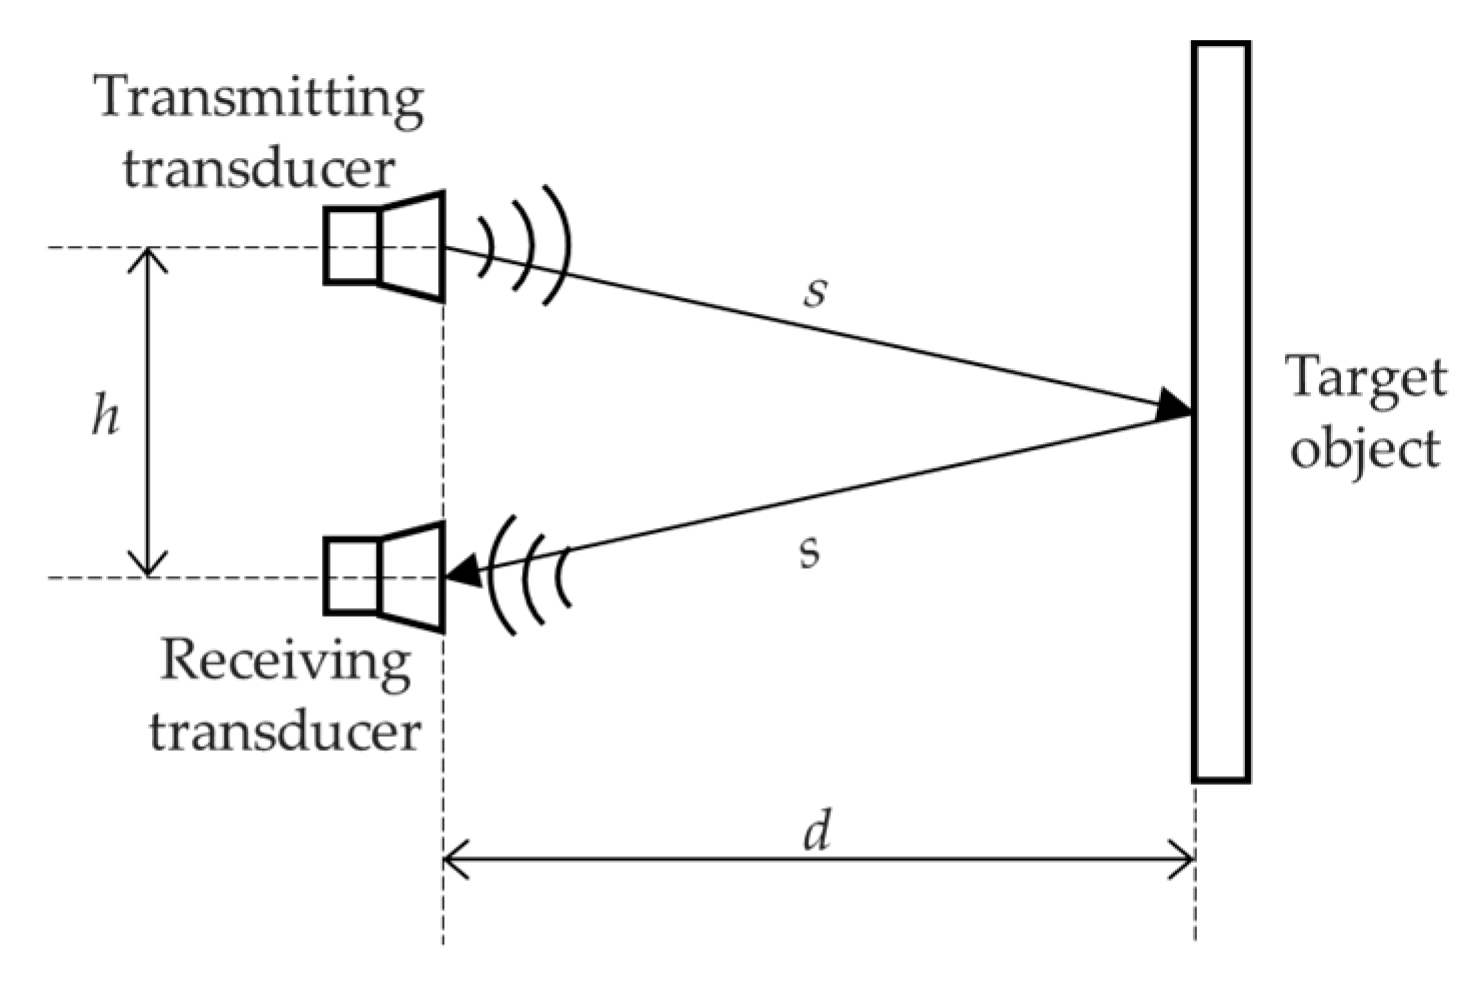
\includegraphics[width=0.95\linewidth]{figures/schematic_diagram_for_pair_of_transducer.png}
\caption{Pitch-catch ultrasonic ranging geometry (adapted from \cite{mi13040520}).}
\label{fig:pitch_catch_mode}
\end{figure}

\subsection{Speed of Sound in Air and Environmental Compensation}

The speed of sound in air depends primarily on the ambient
temperature. In dry air at $0^\circ$C, the speed of sound is
approximately

\begin{equation}
c \approx 331.45 \; \mathrm{m\,s^{-1}}
\end{equation}

A commonly used linear approximation relating sound speed
to air temperature is \cite{mi13040520}

\begin{equation}
c \approx 331.45 + 0.607\,T_C
\end{equation}

where $T_C$ is the air temperature in degrees Celsius. This
relation indicates that the speed of sound increases by about
$0.6\,\mathrm{m\,s^{-1}}$ for every $1^\circ$C increase in
temperature.

Environmental factors such as humidity and atmospheric
pressure also affect the propagation speed of sound, though
their influence is comparatively smaller. Across typical
ranges of $0$--$100\%$ relative humidity and
$50$--$110$\,kPa pressure, the variation in sound speed is
generally less than $0.7\%$ \cite{mi13040520}.

For improved measurement accuracy, the ESP32 can update
distance calculations using a temperature-dependent value
of $c$. If ambient temperature is known, systematic errors
caused by environmental variations can be reduced.


